% Provenance (never printed): see sources/outline_sources.md (Year 3: the main
% field and its secular variation, rock magnetism, palaeomagnetic poles, apparent
% polar wander, magnetostratigraphy, the geodynamo). Brief: sources/book5/BRIEFS.md,
% ch. 4. Curves and maps from figdata/bachelor-3/igrf_field.py (IGRF-14),
% palaeomag_stats.py (the invented Kesta terrane, its Fisher statistics, the
% Zijderveld specimen and the reference APW path), magnetostratigraphy.py.
% Exercise and problem values in the Book 5 scratch calculator calc/ch04.py.
\chapter{Geomagnetismo y paleomagnetismo}\label{ch:b3:palaeomagnetism}

Un flujo basáltico erupcionado hace sesenta millones de años se enfrió con sus diminutos granos de
magnetita fijados paralelos al campo de la época. Hoy, al perforarlo, orientarlo in
situ, cortarlo en cilindros pequeños y calentarlo
paso a paso en una sala apantallada del campo actual, aún indica a qué distancia
del polo se encontraba entonces y hacia dónde miraba. Miles de tales
medidas, procedentes de todos los continentes y de todas las edades, han revelado cómo
se desplazaron los continentes antes de que nacieran los fondos oceánicos que registran su movimiento, y en
qué orden se ha invertido el campo a lo largo de las capas de una serie
sedimentaria. Este capítulo describe el campo tal como es hoy, cómo lo registran las rocas,
cómo se extrae y promedia una dirección, y qué dice un polo paleomagnético
sobre el movimiento de una placa.

\begin{recall}
La Tierra como imán y la declinación magnética están en los volúmenes escolares de los
libros de física; los dominios magnéticos, la histéresis, la remanencia y la
temperatura de Curie en su volumen de tercer año; el campo de un dipolo magnético, en su
volumen de primer año. Las inversiones magnéticas y las polaridades normal e inversa se
vieron en año 11. El círculo máximo y el triángulo esférico se definieron en
el volumen de primer año, en su capítulo de astronomía esférica; el cron de polaridad,
la escala de tiempo de polaridad geomagnética, la anomalía magnética marina y las rotaciones finitas
alrededor de un polo de Euler, en su capítulo de cinemática de placas sobre una esfera;
la traza de punto caliente, en su capítulo sobre puntos calientes. Los armónicos esféricos y
las funciones de Legendre normalizadas de Schmidt $P_n^m$ se usaron para la gravedad en
el capítulo de gravedad y la forma de la Tierra (\cref{ch:b3:gravity-geodesy}).
\end{recall}

\section{El campo principal}

\begin{definition}[Campo geomagnético principal; dipolo axial geocéntrico]\label{def:b3:palaeomagnetism:main-field}
El \emph{campo geomagnético principal}\index{campo geomagnético principal} es la
parte del campo magnético terrestre producida en el interior de la Tierra, en su
núcleo externo líquido de hierro; cambia de años a millones de años, a diferencia de los campos de la
ionosfera y la magnetosfera, que cambian en segundos a días. El
\emph{dipolo axial geocéntrico}\index{dipolo axial geocéntrico} es el campo de un
dipolo magnético situado en el centro de la Tierra y alineado
con su eje de rotación, apuntando al sur, de modo que sus líneas de campo salen del hemisferio sur y
entran en el norte.
\end{definition}

En cada punto de la superficie el campo $\mathbf F$ es un vector. Se describe
en un sistema local (figura de abajo): $X$ hacia el norte geográfico, $Y$ hacia el
este, $Z$ hacia abajo. Su componente horizontal es $H = \sqrt{X^2 + Y^2}$, su
intensidad total $F = |\mathbf F|$, su declinación magnética $D$, el ángulo desde
el norte geográfico hasta $\mathbf H$, medido en sentido horario, y su inclinación $I$, el
ángulo desde la horizontal hasta $\mathbf F$.

\begin{definition}[Inclinación magnética]\label{def:b3:palaeomagnetism:inclination}
La \emph{inclinación magnética}\index{inclinación magnética} $I$ del campo en
un punto es el ángulo entre el vector campo y el plano horizontal,
positivo cuando el campo apunta hacia abajo: $\tan I = Z/H$, con $-\ang{90} \le I
\le \ang{90}$.
\end{definition}

\begin{omfigure}
\begin{tikzpicture}[font=\small, x=1cm, y=1cm, >={Stealth[length=5pt]}]
% schematic; X = 3.0, Y = 1.0 (along the oblique east axis), Z = 2.4
\coordinate (O) at (0,0);
\coordinate (E) at (0.9,0.65);
\fill[gray!12] (-0.6,-0.43) -- (3.6,-0.43) -- ($(3.6,-0.43)+2.2*(E)$) -- ($(-0.6,-0.43)+2.2*(E)$) -- cycle;
\draw[->] (O) -- (4.0,0) node[right] {$X$, norte geográfico};
\draw[->] (O) -- ($1.9*(E)$) node[above right] {$Y$, este};
\draw[->] (O) -- (0,-3.0) node[below] {$Z$, abajo};
\coordinate (Hh) at ($(3.0,0)+1.0*(E)$);
\coordinate (F) at ($(Hh)+(0,-2.4)$);
\draw[densely dashed, gray] (3.0,0) -- (Hh);
\draw[densely dashed, gray] ($1.0*(E)$) -- (Hh);
\draw[densely dashed, gray] (Hh) -- (F);
\draw[densely dashed, gray] (0,-2.4) -- (F);
\draw[very thick, ->, blue!60!black] (O) -- (Hh) node[pos=0.3, above, sloped] {$\mathbf H$};
\draw[very thick, ->, red!70!black] (O) -- (F) node[pos=0.55, below left] {$\mathbf F$};
\draw[thick] (1.25,0) arc[start angle=0, end angle=9.46, radius=1.25];
\node at (1.62,0.13) {$D$};
\draw[thick, red!70!black] ($0.36*(Hh)$) to[bend left=30] ($0.3*(F)$);
\node[red!70!black] at (1.62,-0.42) {$I$};
\end{tikzpicture}

\par\smallskip{\small Los elementos del campo en un punto: componentes norte $X$, este
$Y$ y abajo $Z$, la componente horizontal $\mathbf H$, el campo total
$\mathbf F$, la declinación magnética $D$ (en el plano horizontal, en gris)
y la inclinación $I$ (en el plano vertical que contiene a $\mathbf
F$).}\label{fig:b3:palaeomagnetism:elements}
\end{omfigure}

\begin{theorem}[La fórmula del dipolo]\label{thm:b3:palaeomagnetism:dipole}
En la superficie de una esfera de radio $a$, el campo de un \omterm{def:b3:palaeomagnetism:main-field}{dipolo axial geocéntrico}
de momento $m$ tiene, a la latitud $\lambda$,
\[
  H = B_0\cos\lambda,\qquad Z = 2B_0\sin\lambda,\qquad
  F = B_0\sqrt{1 + 3\sin^2\lambda},\qquad
  \tan I = 2\tan\lambda,\qquad D = 0,
\]
donde $B_0 = \mu_0 m/(4\pi a^3)$ es el campo en el ecuador. Esta es la
\emph{fórmula del dipolo}\index{fórmula del dipolo}.
\end{theorem}

\begin{proof}
Fuera de sus fuentes, el campo deriva de un potencial escalar magnético,
$\mathbf B = -\nabla V$. Para un dipolo de momento $m$ que apunta a lo largo de $-z$, el
sur geográfico, $V = -\mu_0 m\cos\theta/(4\pi r^2)$, con $\theta$ la
colatitud. En coordenadas esféricas, $B_r = -\partial V/\partial r =
-2\mu_0 m\cos\theta/(4\pi r^3)$ y $B_\theta = -(1/r)\,\partial V/\partial\theta =
-\mu_0 m\sin\theta/(4\pi r^3)$, y $B_\varphi = 0$. En $r = a$, la componente hacia abajo
es $Z = -B_r = 2B_0\cos\theta = 2B_0\sin\lambda$, y como
$\mathbf e_\theta$ apunta al sur, la componente hacia el norte es $X = -B_\theta =
B_0\sin\theta = B_0\cos\lambda$, con $Y = 0$. Entonces $H = X$, $D = 0$, $\tan I =
Z/H = 2\tan\lambda$ y $F^2 = B_0^2(\cos^2\lambda + 4\sin^2\lambda) =
B_0^2(1 + 3\sin^2\lambda)$.
\end{proof}

La inclinación es cero en el ecuador, \ang{90} en el polo norte, y
negativa en el hemisferio sur; la intensidad es el doble en los polos que en el
ecuador. El campo real no es un dipolo perfecto y se describe, como la gravedad,
mediante armónicos esféricos.

\begin{definition}[Campo Geomagnético Internacional de Referencia]\label{def:b3:palaeomagnetism:igrf}
El \emph{Campo Geomagnético Internacional de Referencia}\index{Campo Geomagnético Internacional de Referencia}
(IGRF) es el modelo acordado internacionalmente del
campo principal: el potencial, en la superficie y por encima de ella,
\[
  V(r,\theta,\varphi) = a\sum_{n=1}^{N}\Bigl(\frac ar\Bigr)^{n+1}\sum_{m=0}^{n}
  \bigl(g_n^m\cos m\varphi + h_n^m\sin m\varphi\bigr)P_n^m(\cos\theta),
\]
con $a = \qty{6371.2}{km}$, $\mathbf B = -\nabla V$, y coeficientes de Gauss
$g_n^m$, $h_n^m$ (en \unit{nT}) que se publican cada cinco años desde 1900, junto
con su tasa de variación en los cinco años siguientes.
\end{definition}
% ledger: geomag5:igrf, data:b5-igrf

El modelo lo mantiene la Asociación Internacional de Geomagnetismo y
Aeronomía; su decimocuarta generación se completó en noviembre de 2024 y se
trunca en el grado $N = 13$. El primer término, $g_1^0$, es el dipolo axial:
comparando con la demostración anterior, $B_0 = -g_1^0$, y $g_1^0 = \qty{-29350}{nT}$
en 2025. Con los otros dos términos de grado 1 el dipolo está inclinado; su eje corta
la superficie en el polo geomagnético norte, en \ang{80.79}\,N, \ang{72.76}\,O en
2025, y su momento es $m = 4\pi a^3\sqrt{(g_1^0)^2 + (g_1^1)^2 +
(h_1^1)^2}/\mu_0 = \qty{7.69e22}{A.m^2}$.
% ledger: data:b5-igrf

\begin{omfigure}
\begin{tikzpicture}
\begin{groupplot}[group style={group size=1 by 2, vertical sep=1.4cm},
  ommap, width=0.96\linewidth, xtick={-180,-120,...,180}, ytick={-60,0,60},
  unbounded coords=jump, title style={font=\small, yshift=-1ex}]
\nextgroupplot[title={(a) inclinación, cada \ang{20}}]
% computed in figdata/bachelor-3/igrf_field.py; ledger: data:b5-igrf, data:ne-land
\addplot[fill=omLithAlluv, draw=black!45, line width=0.2pt, forget plot] table {figdata/out/shared-geo-land.dat};
\addplot[red!70!black, line width=0.5pt] table[x=x, y=y] {figdata/out/bachelor-3-igrf_field-incl.dat};
\addplot[black, line width=1.1pt] table[x=x, y=y] {figdata/out/bachelor-3-igrf_field-dipeq.dat};
\addplot[draw=none, nodes near coords, point meta=explicit,
  every node near coord/.style={font=\tiny, fill=white, inner sep=0.6pt, anchor=center}]
  table[x=x, y=y, meta=lev] {figdata/out/bachelor-3-igrf_field-inclab.dat};
\nextgroupplot[title={(b) intensidad total, cada \qty{5000}{nT}}]
\addplot[fill=omLithAlluv, draw=black!45, line width=0.2pt, forget plot] table {figdata/out/shared-geo-land.dat};
\addplot[blue!60!black, line width=0.5pt] table[x=x, y=y] {figdata/out/bachelor-3-igrf_field-intens.dat};
\addplot[draw=none, nodes near coords, point meta=explicit,
  every node near coord/.style={font=\tiny, fill=white, inner sep=0.6pt, anchor=center}]
  table[x=x, y=y, meta=lev] {figdata/out/bachelor-3-igrf_field-intlab.dat};
\addplot[only marks, mark=x, mark size=3pt, line width=1pt, black] table {figdata/out/bachelor-3-igrf_field-fmin.dat};
\end{groupplot}
\end{tikzpicture}

\par\smallskip{\small El campo principal en 2025 según el decimocuarto IGRF, en la
superficie de la esfera de radio \qty{6371.2}{km}. (a) Inclinación en grados;
la línea gruesa, $I = 0$, es el ecuador de buzamiento cero. (b) Intensidad total en \unit{nT};
la cruz marca el campo más débil, unas \qty{22100}{nT}, sobre el Atlántico
Sur, frente a unas \qty{66600}{nT} en el más intenso, al sur de
Australia.}\label{fig:b3:palaeomagnetism:igrf-maps}
\end{omfigure}

Los mapas anteriores muestran cuánto se aparta el campo de un dipolo. El ecuador de
buzamiento cero se desplaza hasta unos \ang{12} respecto al ecuador geográfico, y la
intensidad, que un dipolo haría uniforme a lo largo de un paralelo, varía en un factor de
tres, con una amplia zona de baja intensidad sobre el Atlántico Sur.
% ledger: data:b5-igrf

\begin{definition}[Variación secular]\label{def:b3:palaeomagnetism:secular}
La \emph{variación secular}\index{variación secular} es el cambio lento del
campo principal con el tiempo, a lo largo de años a siglos, y se mide mediante la
tasa de variación de sus coeficientes de Gauss o de sus elementos en un lugar.
\end{definition}

En los últimos 125 años el momento dipolar ha descendido de
\qty{8.32e22}{A.m^2} a \qty{7.69e22}{A.m^2}, un \qty{7.6}{\percent}, y el polo geomagnético norte
se ha desplazado de \ang{78.61}\,N, \ang{68.79}\,O a su posición actual
(figura inferior); $g_1^0$ sigue creciendo \qty{12.6}{nT} al año, lo que
indica un debilitamiento del dipolo.
% ledger: data:b5-igrf

\begin{omfigure}
\begin{tikzpicture}
\begin{groupplot}[group style={group size=2 by 1, horizontal sep=1.7cm},
  omrecord, width=0.47\linewidth, height=0.4\linewidth, xmin=1895, xmax=2030,
  xtick={1900,1950,2000}, xticklabel style={/pgf/number format/1000 sep=},
  xlabel={año}]
\nextgroupplot[ylabel={momento dipolar (\qty{e22}{A.m^2})}, ymin=7.6, ymax=8.4]
% computed in figdata/bachelor-3/igrf_field.py; ledger: data:b5-igrf
\addplot[omDef, thick, mark=*, mark size=1pt] table[x=year, y=M] {figdata/out/bachelor-3-igrf_field-dipole.dat};
\nextgroupplot[ylabel={latitud del polo (\unit{\degree}\,N)}, ymin=78, ymax=81.5]
\addplot[red!70!black, thick, mark=*, mark size=1pt] table[x=year, y=plat] {figdata/out/bachelor-3-igrf_field-dipole.dat};
\end{groupplot}
\end{tikzpicture}

\par\smallskip{\small La parte dipolar del campo principal, 1900--2025, cada cinco
años, según el IGRF: su momento (izquierda) y la latitud del polo geomagnético
norte (derecha).}\label{fig:b3:palaeomagnetism:dipole}
\end{omfigure}

¿De dónde procede el campo? Un imán permanente queda descartado: la temperatura de Curie
de la magnetita es de unos \qty{580}{\celsius} y la de la hematites
\qty{675}{\celsius}, y el interior de la Tierra está mucho más caliente. El campo
se regenera de forma continua por el movimiento del líquido conductor del núcleo
externo.
% ledger: tarduno:curie

\begin{definition}[Geodinamo]\label{def:b3:palaeomagnetism:geodynamo}
La \emph{geodinamo}\index{geodinamo} es el proceso autosostenido mediante el cual
la convección de la aleación de hierro líquida y conductora de la electricidad del núcleo
externo, desviada por la rotación de la Tierra, induce corrientes eléctricas cuyo
campo magnético se mantiene frente a la disipación óhmica.
\end{definition}

\begin{proposition}[Ecuación de inducción]\label{prop:b3:palaeomagnetism:induction}
En un conductor de difusividad magnética $\eta = 1/(\mu_0\sigma)$ que se mueve con la
velocidad $\mathbf u$, el campo magnético obedece
\[
  \frac{\partial\mathbf B}{\partial t} = \nabla\times(\mathbf u\times\mathbf B)
  + \eta\nabla^2\mathbf B .
\]
\end{proposition}
\admitted

El primer término estira y retuerce las líneas de campo arrastradas por el flujo; el
segundo hace que el campo decaiga, en un cuerpo de tamaño $L$, en un tiempo del orden de
$L^2/\eta$. Un dinamo funciona cuando el flujo regenera el campo más deprisa de lo que este
se difunde. Las simulaciones numéricas de una envoltura de fluido en convección y rotación
reproducen un dipolo axial dominante y, de vez en cuando, una inversión; pero las
ecuaciones de la \omterm{def:b3:palaeomagnetism:geodynamo}{geodinamo}, acopladas con las del flujo, quedan fuera de este
libro. Además de las inversiones completas, el registro contiene episodios más breves.

\begin{definition}[Excursión geomagnética]\label{def:b3:palaeomagnetism:excursion}
Una \emph{excursión geomagnética}\index{excursión geomagnética} es una desviación grande
de la dirección del campo respecto a la del dipolo axial, el
\omterm{def:b3:palaeomagnetism:vgp}{polo geomagnético virtual} (véase la \cref{def:b3:palaeomagnetism:vgp}) que se aleja mucho del
polo geográfico, y el campo vuelve a la polaridad original en lugar de
completar una inversión.
\end{definition}

\section{Cómo registran las rocas el campo}

Los minerales ferromagnéticos en sentido amplio, principalmente la magnetita en las rocas ígneas
y la hematites en los sedimentos rojos, portan una remanencia. Por encima de su temperatura de Curie
un grano no tiene ninguna; por debajo de ella, un grano pequeño es un único dominio magnético cuyo
momento cambia de sentido entre sus direcciones de fácil imanación, activado térmicamente, tras un
tiempo de relajación
\[
  \tau = \frac1C\exp\Bigl(\frac{K V}{k_B T}\Bigr),
\]
donde $K$ es la energía de anisotropía por unidad de volumen, $V$ el volumen del grano
y $C$ un factor de frecuencia. Esta es la ley de relajación de Néel, admitida aquí. Como
$\tau$ crece exponencialmente al disminuir $T$, un grano pasa en un intervalo estrecho
de temperatura desde cambiar libremente de sentido a retener su momento durante miles de millones de
años.

\begin{definition}[Temperatura de bloqueo]\label{def:b3:palaeomagnetism:blocking}
La \emph{temperatura de bloqueo}\index{temperatura de bloqueo} de un grano magnético
es la temperatura por debajo de la cual su tiempo de relajación supera el tiempo del
experimento, de modo que su momento permanece fijo: al enfriarse a través de ella, el grano
registra el campo; al calentarse a través de ella en campo nulo, el grano pierde ese
registro.
\end{definition}

\begin{definition}[Magnetización remanente natural, térmica, detrítica y química]\label{def:b3:palaeomagnetism:nrm}
La \emph{magnetización remanente natural}\index{magnetización remanente natural}
(NRM) de una roca es la remanencia que conserva al recogerse, la suma de
componentes adquiridas en distintos momentos. Una \emph{magnetización
termorremanente}\index{magnetización termorremanente} (TRM) se adquiere al enfriarse
a través de las \omterm{def:b3:palaeomagnetism:blocking}{temperaturas de bloqueo} en un campo, como en una colada de lava o en una
intrusión. Una \emph{magnetización remanente detrítica}\index{magnetización remanente detrítica}
(DRM) se adquiere cuando los granos magnéticos que sedimentan en agua, o en
el sedimento húmedo justo debajo de su superficie, se orientan con el campo antes de
quedar fijados. Una \emph{magnetización remanente química}\index{magnetización remanente química}
(CRM) se adquiere cuando un mineral magnético crece, a través de un
volumen de bloqueo, en un campo, como hace la hematites al formarse un lecho rojo.
\end{definition}

La TRM registra el campo en el momento del enfriamiento; la DRM, en el tiempo que
tarda el sedimento en compactarse; la CRM, cuando creció el mineral, lo que puede ser mucho
después de la sedimentación. Un calentamiento posterior, o el campo actual actuando durante mucho tiempo
sobre granos de relajación breve, añade una componente secundaria encima: una
remanencia viscosa a lo largo del campo reciente.

\section{De una muestra a una dirección}

Se perforan testigos orientados en varios puntos de una formación, unos pocos testigos por
punto, y se cortan en muestras de unos pocos centímetros cúbicos. Se mide la NRM de cada muestra
y después se elimina progresivamente.

\begin{definition}[Desmagnetización por pasos]\label{def:b3:palaeomagnetism:demag}
La \emph{desmagnetización por pasos}\index{desmagnetización por pasos} es la eliminación
de la remanencia de una muestra en etapas de intensidad creciente, midiendo el
vector remanente tras cada una: calentando a temperaturas crecientes y enfriando
en campo nulo (desmagnetización térmica), que elimina primero las componentes de
menor \omterm{def:b3:palaeomagnetism:blocking}{temperatura de bloqueo}, o mediante campos magnéticos alternos de valor pico creciente
que decaen hasta cero (desmagnetización por campo alterno), que elimina primero
las de menor coercitividad.
\end{definition}

\begin{definition}[Diagrama de Zijderveld; magnetización remanente característica]\label{def:b3:palaeomagnetism:zijderveld}
Un \emph{diagrama de Zijderveld}\index{diagrama de Zijderveld} representa los extremos del
vector de remanencia restante tras cada paso de desmagnetización en dos planos
a la vez, el horizontal (norte frente a este) y uno vertical (norte
frente a abajo), con un eje norte común. Una componente eliminada sola en un intervalo
de pasos se representa como un segmento recto; un segmento que termina en el origen es la
\emph{magnetización remanente característica}\index{magnetización remanente característica}
(ChRM), la componente más estable, que se interpreta como la primaria
cuando los ensayos lo permiten.
\end{definition}

La muestra de la figura siguiente porta dos componentes: una sobreimpresión viscosa
a lo largo del campo actual, eliminada a \qty{300}{\celsius}, y una componente ChRM
que se desbloquea desde 300 hasta \qty{580}{\celsius}, la temperatura de Curie de la magnetita.
Por encima de \qty{300}{\celsius} ambas proyecciones llegan en línea recta al origen; la
dirección de ese segmento es la de la ChRM.

\begin{omfigure}
\begin{tikzpicture}
\begin{groupplot}[group style={group size=2 by 1, horizontal sep=1.3cm},
  width=0.5\linewidth]
\nextgroupplot[axis lines=middle, axis equal image, xmin=-4, xmax=36, ymin=-4, ymax=42,
  y dir=reverse, xlabel={N}, ylabel={E, abajo}, tick label style={font=\scriptsize},
  xtick={0,10,20,30}, ytick={10,20,30,40}, label style={font=\small},
  xlabel style={at={(ticklabel* cs:1.0)}, anchor=west},
  ylabel style={at={(ticklabel* cs:1.0)}, anchor=north west},
  title={(a) Diagrama de Zijderveld (\unit{mA/m})}, title style={font=\small, yshift=1ex},
  clip=false, legend style={font=\scriptsize, at={(0.13,0.03)}, anchor=south west, cells={anchor=west}}]
% computed in figdata/bachelor-3/palaeomag_stats.py (synthetic specimen)
\addplot[black, mark=*, mark size=1.5pt] table[x=N, y=E] {figdata/out/bachelor-3-palaeomag_stats-zij.dat};
\addlegendentry{horizontal: N, E}
\addplot[black, mark=o, mark size=1.7pt, fill=white] table[x=N, y=Down] {figdata/out/bachelor-3-palaeomag_stats-zij.dat};
\addlegendentry{vertical: N, abajo}
\node[font=\scriptsize, anchor=south west] at (axis cs:32.2,18.1) {\qty{20}{\celsius}};
\node[font=\scriptsize, anchor=north west] at (axis cs:32.2,38.2) {\qty{20}{\celsius}};
\node[font=\scriptsize, anchor=south] at (axis cs:25.8,17.6) {300};
\node[font=\scriptsize, anchor=east] at (axis cs:25.0,24.6) {300};
\node[font=\scriptsize, anchor=south east] at (axis cs:-0.5,-0.5) {580};
\nextgroupplot[axis equal image, hide axis, clip=false, xmin=-1.12, xmax=1.12, ymin=-1.12, ymax=1.18,
  title={(b) sitio A, proyección de igual área, hemisferio inferior}, title style={font=\small, yshift=1ex}]
\addplot[black, domain=0:360, samples=145, thin] ({cos(x)},{sin(x)});
\draw[black] (axis cs:0,1) -- (axis cs:0,1.08) node[above, font=\scriptsize] {N};
\draw[black] (axis cs:1,0) -- (axis cs:1.06,0);
\draw[black] (axis cs:0,-1) -- (axis cs:0,-1.06);
\draw[black] (axis cs:-1,0) -- (axis cs:-1.06,0);
\draw[black] (axis cs:-0.04,0) -- (axis cs:0.04,0) (axis cs:0,-0.04) -- (axis cs:0,0.04);
\addplot[only marks, mark=*, mark size=1.6pt, black] table[x=x, y=y] {figdata/out/bachelor-3-palaeomag_stats-dirsA.dat};
\addplot[omDef, thick] table[x=x, y=y] {figdata/out/bachelor-3-palaeomag_stats-cone.dat};
\addplot[only marks, mark=star, mark size=3.5pt, omDef, line width=0.9pt] table[x=x, y=y] {figdata/out/bachelor-3-palaeomag_stats-meanA.dat};
\end{groupplot}
\end{tikzpicture}

\par\smallskip{\small (a) Desmagnetización térmica de una muestra sintética, desde
\qty{20}{\celsius} a \qty{580}{\celsius}: puntos rellenos, la horizontal
proyección; puntos vacíos, la vertical. (b) Las seis direcciones de la ChRM del sitio A
del problema de fin de semana (puntos), su media (estrella) y su cono de
confianza al 95 por ciento (círculo).}\label{fig:b3:palaeomagnetism:zijderveld}
\end{omfigure}

Las direcciones de las muestras de un sitio se dispersan alrededor de una media, y la
estadística de esa dispersión es la de una distribución sobre la esfera.

\begin{proposition}[Distribución de Fisher]\label{prop:b3:palaeomagnetism:fisher}
La \emph{distribución de Fisher}\index{distribución de Fisher} de precisión
parámetro $\kappa > 0$ alrededor de una dirección media asigna a un vector unitario la
densidad de probabilidad, por unidad de ángulo sólido,
\[
  f(\theta) = \frac{\kappa}{4\pi\sinh\kappa}\,e^{\kappa\cos\theta},
\]
donde $\theta$ es su ángulo respecto de la media. Dados $N$ vectores unitarios $\mathbf u_i$
extraídos de ella, con resultante $\mathbf R = \sum\mathbf u_i$ de longitud $R$, la
mejor estimación de la dirección media es la de $\mathbf R$; la precisión se
estima mediante $k = (N - 1)/(N - R)$; y la media verdadera se encuentra, con probabilidad
$1 - p$, dentro del ángulo $\alpha_{1-p}$ de la media estimada, donde
\[
  \cos\alpha_{1-p} = 1 - \frac{N - R}{R}\Bigl[\Bigl(\frac1p\Bigr)^{1/(N-1)} - 1\Bigr].
\]
\end{proposition}
\admitted

\begin{definition}[Alfa-95]\label{def:b3:palaeomagnetism:a95}
El \emph{alfa-95}\index{alfa-95} ($\alpha_{95}$) de una dirección media es el
semiángulo de su cono de confianza al 95 por ciento, el ángulo $\alpha_{1-p}$ de
la \cref{prop:b3:palaeomagnetism:fisher} para $p = 0.05$.
\end{definition}

La densidad se integra a uno: con $\mathrm d\Omega = 2\pi\sin\theta\,\mathrm
d\theta$, $\int_0^\pi f\,2\pi\sin\theta\,\mathrm d\theta =
\frac{\kappa}{2\sinh\kappa}\cdot\frac{e^\kappa - e^{-\kappa}}{\kappa} = 1$. Las direcciones se promedian como vectores unitarios
nunca como ángulos: la media de las declinaciones \ang{350} y \ang{10} es
el norte, no el sur. Un $k$ grande significa un agrupamiento estrecho, y $\alpha_{95}$ disminuye
aproximadamente como $1/\sqrt{kN}$.

\begin{method}[Pruebas de campo de una dirección paleomagnética]\label{met:b3:palaeomagnetism:tests}
Puede demostrarse que una ChRM es anterior a un evento mediante una prueba realizada en el campo.
\begin{itemize}
  \item \textbf{Prueba del pliegue.} Sitios en ambos flancos de un pliegue: si las direcciones
        se agrupan mejor después de devolver los estratos a la horizontal que antes,
        la magnetización es anterior al plegamiento.
  \item \textbf{Prueba de inversión.} Si una formación contiene ambas polaridades, la media
        de las direcciones inversas, una vez invertida, debe coincidir con la media de
        las normales dentro de sus conos de confianza; una sobreimpresión viscosa no
        eliminada sesgaría ambas en el mismo sentido y rompería la antipodalidad.
  \item \textbf{Prueba del contacto cocido.} Un dique calienta la roca encajante junto a él,
        que adquiere una nueva TRM: si la roca cocida conserva la dirección del dique y
        la roca encajante más alejada presenta otra distinta, la magnetización del dique
        no se ha reseteado desde que se enfrió.
\end{itemize}
\end{method}

\section{Polos y placas}

Si el campo, promediado a lo largo de unos pocos miles de años para suavizar la
\omterm{def:b3:palaeomagnetism:secular}{variación secular}, es un \omterm{def:b3:palaeomagnetism:main-field}{dipolo axial geocéntrico}, entonces la \omterm{thm:b3:palaeomagnetism:dipole}{fórmula del dipolo} convierte una
inclinación media en una latitud, y la declinación media apunta al polo.

\begin{definition}[Paleolatitud; polo geomagnético virtual]\label{def:b3:palaeomagnetism:vgp}
La \emph{paleolatitud}\index{paleolatitud} de un sitio es la latitud
$\lambda$ dada por su inclinación media mediante la \omterm{thm:b3:palaeomagnetism:dipole}{fórmula del dipolo}, $\tan I =
2\tan\lambda$. El \emph{polo geomagnético virtual}\index{polo geomagnético virtual}
(VGP, por sus siglas en inglés) de una dirección $(D, I)$ observada en un sitio es el polo
norte del dipolo geocéntrico que produciría esa dirección allí.
\end{definition}

\begin{theorem}[El polo de una dirección]\label{thm:b3:palaeomagnetism:pole}
Sea un sitio de latitud $\lambda_s$ y longitud $\varphi_s$ y una dirección media
$(D, I)$. Sea $p$ la paleocolatitud, $\cot p = \tfrac12\tan I$,
con $0 \le p \le \ang{180}$. El \omterm{def:b3:palaeomagnetism:vgp}{polo geomagnético virtual} tiene latitud
$\lambda_p$ y longitud $\varphi_p$ dadas por
\[
  \sin\lambda_p = \sin\lambda_s\cos p + \cos\lambda_s\sin p\cos D,\qquad
  \sin\beta = \frac{\sin p\sin D}{\cos\lambda_p},
\]
con $\varphi_p = \varphi_s + \beta$ si $\cos p \ge \sin\lambda_s\sin\lambda_p$,
y $\varphi_p = \varphi_s + \ang{180} - \beta$ en caso contrario.
\end{theorem}

\begin{proof}
Sobre la esfera, el sitio $S$, el polo norte geográfico $N$ y el VGP $P$ forman un
triángulo esférico (figura siguiente). El lado $NS$ es la colatitud del sitio,
$\ang{90} - \lambda_s$; el lado $SP$ es la distancia angular desde el sitio al
polo del dipolo, que la \omterm{thm:b3:palaeomagnetism:dipole}{fórmula del dipolo} da como $p$, puesto que la latitud
magnética del sitio es $\ang{90} - p$; y el ángulo en $S$, entre las
direcciones hacia $N$ y hacia $P$, es la declinación $D$. La regla del coseno para el
lado $NP = \ang{90} - \lambda_p$ da la primera relación; la regla del seno,
$\sin\beta/\sin p = \sin D/\sin(\ang{90} - \lambda_p)$, da el ángulo $\beta$
en $N$, la diferencia de longitudes. El seno fija $\beta$ solo salvo su
suplementario: la regla del coseno para el lado $SP$, $\cos p = \sin\lambda_s
\sin\lambda_p + \cos\lambda_s\cos\lambda_p\cos\beta$, muestra que $\cos\beta \ge
0$ exactamente cuando $\cos p \ge \sin\lambda_s\sin\lambda_p$.
\end{proof}

\begin{omfigure}
\begin{tikzpicture}[font=\small, >={Stealth[length=5pt]}]
\draw[gray!60] (0,0) circle (2.6);
\draw[gray!50, densely dashed] (-2.6,0) arc[start angle=180, end angle=360, x radius=2.6, y radius=0.7];
\coordinate (N) at (0,2.6);
\coordinate (S) at (-1.2,0.25);
\coordinate (P) at (1.25,1.65);
\fill (N) circle (1.6pt) node[above] {$N$};
\fill (S) circle (1.6pt) node[below left] {$S$ (sitio)};
\fill[omDef] (P) circle (1.8pt) node[right] {$P$ (VGP)};
\draw[thick] (N) to[bend right=12] node[left, pos=0.55] {$\ang{90}-\lambda_s$} (S);
\draw[thick, omDef] (S) to[bend left=10] node[below right, pos=0.55] {$p$} (P);
\draw[thick, blue!60!black] (N) to[bend left=12] node[above right, pos=0.45] {$\ang{90}-\lambda_p$} (P);
\draw ($(S)!0.2!(N)$) to[bend left=35] ($(S)!0.2!(P)$);
\node[inner sep=1pt] at (-0.61,0.86) {$D$};
\draw ($(N)!0.18!(S)$) to[bend right=40] node[below, pos=0.5, inner sep=2pt] {$\beta$} ($(N)!0.18!(P)$);
\end{tikzpicture}

\par\smallskip{\small El triángulo esférico del \omterm{def:b3:palaeomagnetism:vgp}{polo geomagnético virtual}:
polo geográfico norte $N$, sitio $S$, polo $P$. El ángulo en el sitio es la
declinación $D$; el ángulo en el polo $N$ es la diferencia de longitudes
$\beta$.}\label{fig:b3:palaeomagnetism:vgp}
\end{omfigure}

El cono $\alpha_{95}$ alrededor de la dirección media se convierte en un óvalo alrededor del polo,
de semiejes $\mathrm dp = \tfrac12\alpha_{95}(1 + 3\cos^2p)$ a lo largo del círculo máximo
desde el sitio, y $\mathrm dm = \alpha_{95}\sin p/\cos I$ a través de él. Un
polo promediado sobre varios sitios de una formación, cada uno un VGP, es un polo paleomagnético
con su propio cono, $A_{95}$. Las rocas de la misma edad sobre una misma placa rígida dan el
mismo polo; rocas de edades distintas, polos distintos.

\begin{definition}[Deriva polar aparente; curva de deriva polar aparente]\label{def:b3:palaeomagnetism:apw}
La \emph{deriva polar aparente}\index{deriva polar aparente} es el cambio, con
la edad de las rocas, del polo paleomagnético de una placa visto desde esa placa,
considerada fija. Una \emph{curva de deriva polar aparente}\index{curva de deriva polar aparente}
es la línea que une los polos paleomagnéticos de una placa en orden
de edad.
\end{definition}

El polo no se desplaza: la placa es la que se mueve, y la curva registra ese movimiento
en sentido inverso. Dos placas que se han separado tienen curvas distintas para el tiempo
anterior a su separación, y cada curva se hace coincidir con la otra mediante la
rotación finita que cierra el océano entre ellas. Un polo paleomagnético fija la
latitud de un bloque y su orientación, pero no su longitud: una rotación del
bloque alrededor del eje de rotación no cambia ni una cosa ni otra.

Un bloque desplazado, un terreno, se contrasta con la curva de la placa estable a la que
pertenece ahora. A partir del polo de referencia de la edad adecuada se calcula la
dirección esperada $(D_x, I_x)$ en el sitio, mediante el \cref{thm:b3:palaeomagnetism:pole}
leído en sentido inverso. Una rotación en sentido horario del bloque alrededor de un eje vertical
se mide con $R = D_o - D_x$, su desplazamiento hacia el polo con $P = \lambda_x -
\lambda_o$, la diferencia entre las \omterm{def:b3:palaeomagnetism:vgp}{paleolatitudes} esperada y observada; el
error de una declinación es de alrededor de $\Delta D = \arcsin(\sin\alpha_{95}/\cos I)$,
y los errores se combinan como la raíz de la suma de sus cuadrados. La cadena de Hawái--Emperador
se sometió a esta prueba en el volumen de primer año, en su capítulo sobre puntos calientes:
las \omterm{def:b3:palaeomagnetism:vgp}{paleolatitudes} medidas en los montes submarinos Emperador mostraron que el propio punto caliente
se desplazaba hacia el sur, en más de \qty{40}{mm/yr} entre 81 y \qty{47}{Ma}.
% ledger: tarduno:emperor

\begin{omfigure}
\begin{tikzpicture}
\begin{axis}[axis equal image, hide axis, width=0.62\linewidth,
  xmin=-0.62, xmax=0.62, ymin=-0.62, ymax=0.62, unbounded coords=jump,
  legend style={font=\scriptsize, at={(1.03,0.5)}, anchor=west, cells={anchor=west}}]
% computed in figdata/bachelor-3/palaeomag_stats.py (invented continent and terrane)
\addplot[gray!50, line width=0.3pt, forget plot] table[x=x, y=y] {figdata/out/bachelor-3-palaeomag_stats-graticule.dat};
\addplot[black, line width=0.6pt, domain=0:360, samples=145, forget plot]
  ({0.5412*cos(x)},{0.5412*sin(x)});
\addplot[draw=none, nodes near coords, point meta=explicit symbolic, forget plot,
  every node near coord/.style={font=\tiny, anchor=center}]
  table[x=x, y=y, meta=lon] {figdata/out/bachelor-3-palaeomag_stats-lonlabels.dat};
\addplot[blue!60!black, line width=0.4pt, forget plot] table[x=x, y=y,
  restrict expr to domain={\thisrow{id}}{0:9}] {figdata/out/bachelor-3-palaeomag_stats-apwcircles.dat};
\addplot[red!70!black, line width=0.4pt, densely dashed, forget plot] table[x=x, y=y,
  restrict expr to domain={\thisrow{id}}{10:19}] {figdata/out/bachelor-3-palaeomag_stats-apwcircles.dat};
\addplot[blue!60!black, thick, mark=square*, mark size=1.6pt] table[x=x, y=y] {figdata/out/bachelor-3-palaeomag_stats-apwref.dat};
\addlegendentry{trayectoria de referencia, continente estable}
\addplot[red!70!black, thick, mark=triangle*, mark size=2.2pt] table[x=x, y=y] {figdata/out/bachelor-3-palaeomag_stats-apwkesta.dat};
\addlegendentry{VGP de Kesta A, B, C}
\node[font=\scriptsize, anchor=west] at (axis cs:0.11,-0.135) {\qty{60}{Ma}};
\node[font=\scriptsize, anchor=west] at (axis cs:0.055,-0.07) {30};
\node[font=\scriptsize, anchor=east] at (axis cs:-0.085,-0.02) {4};
\node[font=\scriptsize, anchor=west] at (axis cs:0.035,0.0) {C, 4};
\node[font=\scriptsize, anchor=west] at (axis cs:-0.09,-0.45) {A, \qty{60}{Ma}};
\node[font=\scriptsize, anchor=west] at (axis cs:-0.04,-0.27) {B, 30};
\fill (axis cs:0,0) circle (1pt);
\end{axis}
\end{tikzpicture}

\par\smallskip{\small Proyección polar de igual área de la región polar norte, hasta
\ang{45}\,N (círculo exterior), paralelos cada \ang{10} desde \ang{50}\,N, meridianos
cada \ang{30} (rotulados en grados este). Cuadrados: la \omterm{def:b3:palaeomagnetism:apw}{curva de deriva polar aparente}
de un continente estable ficticio, con los círculos $A_{95}$ de sus polos;
triángulos: los \omterm{def:b3:palaeomagnetism:vgp}{polos geomagnéticos virtuales} de las tres formaciones del
terreno Kesta ficticio del problema de fin de semana, con sus círculos $\alpha_{95}$
(discontinuos). El polo geográfico es el punto del centro.}\label{fig:b3:palaeomagnetism:apw}
\end{omfigure}

Un polo que se desplaza respecto al eje de rotación puede deberse a que las placas se
hayan movido o a que toda la Tierra sólida haya girado bajo dicho eje.

\begin{definition}[Deriva polar verdadera]\label{def:b3:palaeomagnetism:tpw}
La \emph{deriva polar verdadera}\index{deriva polar verdadera} es la rotación de toda la
Tierra sólida, manto y corteza en conjunto, respecto a su eje de rotación, impulsada
por cambios en la distribución de masa en su interior. Desplaza a la vez todos los
polos paleomagnéticos de todas las placas, mediante la misma rotación, mientras que el
movimiento de las placas desplaza los polos de cada placa de forma distinta.
\end{definition}

Solo se detecta comparando las curvas de todas las placas dentro de un marco
independiente del eje de rotación, como el de los puntos calientes; no se conoce
con certeza qué tan grande ha sido, y aquí no se da ninguna tasa.

\section{Magnetoestratigrafía}

\begin{definition}[Magnetoestratigrafía]\label{def:b3:palaeomagnetism:magnetostratigraphy}
La \emph{magnetoestratigrafía}\index{magnetoestratigrafía} es la subdivisión de una
secuencia de rocas en zonas de polaridad, intervalos de polaridad normal o invertida
uniforme, y la datación de la secuencia al hacer coincidir su patrón de zonas con
el de la escala de tiempo de polaridad geomagnética.
\end{definition}

Una inversión queda registrada, dentro de la resolución del muestreo, en todas partes
en el mismo instante: un límite de inversión en una sección es una superficie isócrona.
Lo que se compara es el patrón de zonas, su número y sus espesores relativos;
una zona aislada podría corresponder a cualquier cron de su misma polaridad. Una o dos
edades independientes, procedentes de una ceniza volcánica o de un fósil, anclan la
correspondencia, y a partir de ahí cada límite de inversión data la sección. En la figura siguiente, una sección de
\qty{64}{m} muestra tres zonas normales; ajustada a los subcronos normales del
cron C2An, de 3.596 a \qty{2.581}{Ma}, sus límites dan una tasa de sedimentación de unos
\qty{40}{m/Myr} por debajo de \qty{20}{m} y de \qty{55}{m/Myr} por encima.
% ledger: iodp:gpts2004

\begin{omfigure}
\begin{tikzpicture}[font=\small, x=1cm, y=1cm]
% section heights (m) and GPTS ages (Ma) as printed: magnetostratigraphy.py, part ties
% section: y = h / 10 cm; timescale: y = (3.8 - t) * 16 cm
\def\hs{0.1}\def\ts{4.2}
\draw (0,0) rectangle (1,6.4);
\foreach \lo/\hi in {4.2/14.8, 19.7/24.6, 29.2/54.0}
  \fill[black] (0,\lo*\hs) rectangle (1,\hi*\hs);
\foreach \h in {0,10,...,60} \draw (0,\h*\hs) -- (-0.12,\h*\hs) node[left, font=\scriptsize] {\h};
 \node[rotate=90, font=\scriptsize] at (-0.95,3.2) {altura en la sección (m)};
 \node[above, align=center, font=\scriptsize] at (0.5,6.45) {sección};
\draw (5,{(3.8-3.8)*\ts}) rectangle (6,{(3.8-2.3)*\ts});
\foreach \a/\b in {3.596/3.330, 3.207/3.116, 3.032/2.581}
  \fill[black] (5,{(3.8-\a)*\ts}) rectangle (6,{(3.8-\b)*\ts});
\foreach \t in {2.4,2.6,...,3.81} \draw (6,{(3.8-\t)*\ts}) -- (6.12,{(3.8-\t)*\ts})
  node[right, font=\scriptsize] {\pgfmathprintnumber[fixed, fixed zerofill, precision=1]{\t}};
 \node[above, align=center, font=\scriptsize] at (5.8,{(3.8-2.3)*\ts+0.05}) {escala temporal, edad (Ma)};
\foreach \h/\t in {4.2/3.596, 14.8/3.330, 19.7/3.207, 24.6/3.116, 29.2/3.032, 54.0/2.581}
  \draw[omDef, densely dashed] (1,\h*\hs) -- (5,{(3.8-\t)*\ts});
\node[font=\scriptsize, anchor=west] at (6.9,{(3.8-2.81)*\ts}) {C2An.1n};
\node[font=\scriptsize, anchor=west] at (6.9,{(3.8-3.16)*\ts}) {C2An.2n};
\node[font=\scriptsize, anchor=west] at (6.9,{(3.8-3.46)*\ts}) {C2An.3n};
\end{tikzpicture}

\par\smallskip{\small Una correlación magnetoestratigráfica: las zonas de polaridad
de una sección ficticia (negro, normal; blanco, inversa) ajustadas a la
escala de tiempo de polaridad entre 3.8 y \qty{2.3}{Ma}. Las líneas discontinuas unen cada
límite de inversión con su edad.}\label{fig:b3:palaeomagnetism:magstrat}
\end{omfigure}

\begin{inthelab}[Laboratorio paleomagnético apantallado]
\begin{minipage}[t]{0.55\linewidth}\vspace{0pt}
El laboratorio es una sala dentro de un blindaje magnético, capas de metal de alta permeabilidad
que reducen el campo terrestre a una pequeña fracción de su valor, de modo que las
muestras no adquieren remanencia nueva mientras se manipulan. Un paleomagnetista
carga las muestras, pequeños cilindros de roca marcados cada uno con una
flecha de orientación, sobre una bandeja larga que las lleva, una tras otra, a un
magnetómetro criogénico, cuyos sensores superconductores, refrigerados con helio líquido,
miden las tres componentes de remanencias mucho más débiles que las que una brújula
podría detectar. Entre medidas, las muestras pasan a un horno apantallado para el siguiente
paso de calentamiento, o por las bobinas de un desmagnetizador de campo alterno
conectado a la misma línea, y el software representa cada \omterm{def:b3:palaeomagnetism:zijderveld}{diagrama de Zijderveld} a medida que
se acumulan los pasos.
\end{minipage}\hfill
\begin{minipage}[t]{0.42\linewidth}\vspace{0pt}
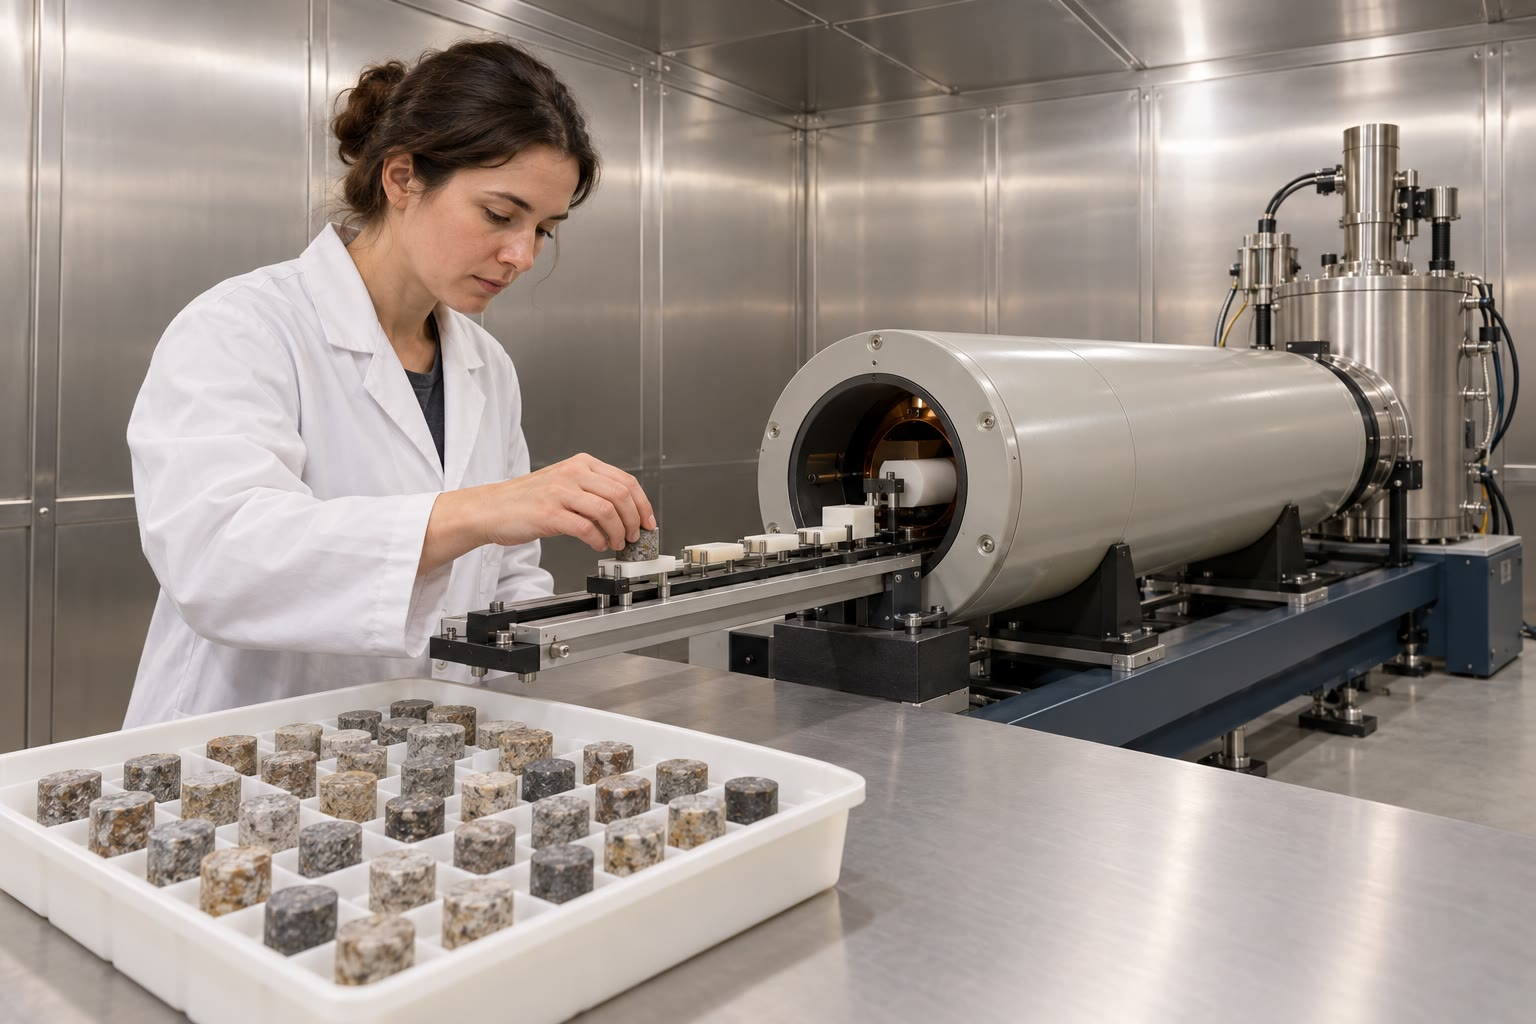
\includegraphics[width=\linewidth]{images/book5/ai/b3-palaeomag-lab.jpg}

{\scriptsize Carga de muestras en la bandeja de un magnetómetro en una
sala apantallada (Ilustración generada por IA.)}
\end{minipage}
\end{inthelab}

\section{Ejercicios}

\begin{exercise}[$\star$]\label{exo:b3:palaeomagnetism:1}
En un campo de \omterm{def:b3:palaeomagnetism:main-field}{dipolo axial geocéntrico}, calcúlese la inclinación a la latitud
\ang{30}\,N, y la latitud de un punto donde la inclinación es \ang{-20}.
\end{exercise}

\begin{exercise}[$\star$]\label{exo:b3:palaeomagnetism:2}
En una estación, el campo tiene componentes $X = \qty{20000}{nT}$, $Y =
\qty{-2000}{nT}$ y $Z = \qty{40000}{nT}$. Calcúlense $H$, $F$, la declinación magnética y la
inclinación.
\end{exercise}

\begin{exercise}[$\star$]\label{exo:b3:palaeomagnetism:3}
En 2025, $g_1^0 = \qty{-29350}{nT}$. Tomando el campo como un dipolo axial,
calcúlense el campo en el ecuador y en los polos, y el momento dipolar
($a = \qty{6371.2}{km}$, $\mu_0 = 4\pi\times\qty{e-7}{H.m^{-1}}$).
\end{exercise}

\begin{exercise}[$\star$]\label{exo:b3:palaeomagnetism:4}
Indíquese el tipo de remanencia adquirida y cuándo registra el campo, en cada uno de los casos: (a) una colada de lava que se enfría;
(b) limo que se deposita en un lago tranquilo; (c) una arenisca cuyos recubrimientos de óxido de hierro
se transforman en hematites durante el enterramiento temprano; (d) un basalto que permanece
durante un millón de años en el campo actual.
\end{exercise}

\begin{exercise}[$\star\star$]\label{exo:b3:palaeomagnetism:5}
Cuatro muestras de una localidad dan las direcciones $(D, I)$: $(\ang{12}, \ang{48})$,
$(\ang{22}, \ang{44})$, $(\ang{16}, \ang{57})$ y $(\ang{6}, \ang{53})$.
Calcúlense sus vectores unitarios, la longitud de la resultante $R$, la dirección media, $k$
y $\alpha_{95}$.
\end{exercise}

\begin{exercise}[$\star\star$]\label{exo:b3:palaeomagnetism:6}
Una localidad en \ang{40.0}\,N, \ang{10.0}\,E da la dirección media $D = \ang{20}$,
$I = \ang{50}$. Calcúlense su \omterm{def:b3:palaeomagnetism:vgp}{paleolatitud} y su \omterm{def:b3:palaeomagnetism:vgp}{polo geomagnético virtual}.
\end{exercise}

\begin{exercise}[$\star\star$]\label{exo:b3:palaeomagnetism:7}
El IGRF da un momento dipolar de \qty{8.32e22}{A.m^2} en 1900 y
\qty{7.69e22}{A.m^2} en 2025, y una tasa de variación de $g_1^0$ de
\qty{+12.6}{nT/yr} en 2025. (a) Calcúlese la variación relativa del momento por
siglo. (b) Si $g_1^0$ mantuviera esa tasa, ¿en cuántos años llegaría a cero?
¿Por qué esto no es una predicción?
\end{exercise}

\begin{exercise}[$\star\star$]\label{exo:b3:palaeomagnetism:8}
La remanencia residual de una muestra, en \unit{mA/m} (norte, este, abajo), es
$(32.2, 18.1, 38.2)$ tras calentar a \qty{20}{\celsius}, $(25.8, 18.1, 24.6)$
tras \qty{300}{\celsius}, y $(0.0, 0.0, 0.0)$ tras \qty{580}{\celsius}; el
\omterm{def:b3:palaeomagnetism:zijderveld}{diagrama de Zijderveld} es recto entre cada par. Calcúlense la dirección y la
intensidad de la componente eliminada entre 20 y \qty{300}{\celsius}, y de la
eliminada por encima de \qty{300}{\celsius}. ¿Cuál es la ChRM y cuál es la
otra?
\end{exercise}

\begin{exercise}[$\star\star$]\label{exo:b3:palaeomagnetism:9}
Una formación da $I = \ang{-35}$ con $\alpha_{95} = \ang{5}$. Calcúlense su
\omterm{def:b3:palaeomagnetism:vgp}{paleolatitud}, el intervalo de \omterm{def:b3:palaeomagnetism:vgp}{paleolatitudes} permitido por $I \pm \alpha_{95}$,
y los semiejes $\mathrm dp$ y $\mathrm dm$ de la elipse de confianza de su
polo.
\end{exercise}

\begin{exercise}[$\star\star\star$]\label{exo:b3:palaeomagnetism:10}
(a) A partir del \cref{thm:b3:palaeomagnetism:dipole}, encuéntrese la latitud en la que
la inclinación es \ang{45}, y la razón entre el campo en los polos y el del
ecuador. (b) Muéstrese que $\mathrm dI/\mathrm d\lambda = 2/(1 + 3\sin^2\lambda)$,
y dedúzcase en qué latitud un error de inclinación produce el mayor error de
\omterm{def:b3:palaeomagnetism:vgp}{paleolatitud}. (c) ¿Por qué las \omterm{def:b3:palaeomagnetism:vgp}{paleolatitudes} obtenidas a partir de inclinaciones bajas son las más
precisas en grados?
\end{exercise}

\begin{exercise}[$\star\star\star$]\label{exo:b3:palaeomagnetism:11}
Un sitio se encuentra en \ang{35.0}\,S, \ang{150.0}\,E, sobre una placa estable cuyo
polo de referencia, para la edad de una formación muestreada allí, está en \ang{70.0}\,N,
\ang{300.0}\,E. (a) Calcúlense la distancia angular $p$ desde el sitio hasta el polo,
la inclinación y la declinación esperadas, y la \omterm{def:b3:palaeomagnetism:vgp}{paleolatitud} esperada.
(b) La formación da $D_o = \ang{30.0}$, $I_o = \ang{-60.0}$. Calcúlense la
rotación $R$ y el desplazamiento hacia el polo $P$, e indíquese qué significan.
\end{exercise}

\begin{exercise}[$\star\star\star$]\label{exo:b3:palaeomagnetism:12}
(a) A partir de la \cref{prop:b3:palaeomagnetism:fisher}, muéstrese que la probabilidad de que
una dirección se encuentre a menos de $\theta$ de la media es $(e^\kappa -
e^{\kappa\cos\theta})/(e^\kappa - e^{-\kappa})$. (b) Para $\kappa$ grande y
$\theta$ pequeño, muéstrese que esta es aproximadamente $1 - e^{-\kappa\theta^2/2}$, y dedúzcase
que \qty{63}{\percent} de las direcciones se encuentra a menos de $\theta_{63} \approx
\ang{81}/\sqrt\kappa$. (c) Calcúlese $\theta_{63}$ para $\kappa = 50$, y compruébese el
\qty{63}{\percent} con la fórmula exacta.
\end{exercise}

\section{Problema: las capas rojas de Kesta}

\begin{problem}[{Problema de fin de semana --- tres formaciones de un terreno desplazado,
sus direcciones, polos y rotaciones, y la edad de la más joven}]
\label{pb:b3:palaeomagnetism:1}
% values: calc/ch04.py; palaeomag_stats.py, magnetostratigraphy.py; GPTS: iodp:gpts2004
Kesta es un terreno inventado, situado hoy en \ang{47.0}\,N, \ang{15.0}\,E, en el borde
de un continente estable inventado. Expone tres formaciones de capas rojas: A,
\qty{60}{Ma}; B, \qty{30}{Ma}; C, de unos 3.7 a \qty{2.4}{Ma}. Cada una fue
muestreada en varios sitios, y cada espécimen fue desmagnetizado térmicamente; la
ChRM está portada por hematites, y las formaciones están dispuestas horizontalmente.

\medskip\noindent\textbf{Parte I --- Direcciones medias.} Los seis sitios de
la formación A dan $(D, I)$: $(\ang{50}, \ang{37})$, $(\ang{28}, \ang{37})$,
$(\ang{21}, \ang{42})$, $(\ang{24}, \ang{27})$, $(\ang{37}, \ang{39})$,
$(\ang{46}, \ang{38})$.
\begin{enumerate}
  \item ¿Por qué puede una ChRM portada por hematites en una capa roja ser más joven que la
        capa? ¿Qué mostraría que no es mucho más joven?
  \item Calcúlese el vector unitario de la primera dirección.
  \item La suma de los seis vectores unitarios es $(3.8943, 2.6500, 3.5717)$. Calcúlense $R$ y
        la dirección media de la formación A.
  \item Calcúlense $k$ y $\alpha_{95}$ para la formación A.
  \item La formación B da, a partir de 7 sitios, $D = \ang{23.9}$, $I = \ang{51.5}$ y
        $R = 6.8979$; la formación C, a partir de 8 sitios, $D = \ang{3.4}$, $I =
        \ang{63.7}$ y $R = 7.8707$. Calcúlense $k$ y $\alpha_{95}$ de cada una.
  \item ¿Qué formación está mejor agrupada? ¿Cuál de las medias está mejor definida?
\end{enumerate}

\medskip\noindent\textbf{Parte II --- Paleolatitudes y polos.}
\begin{enumerate}[resume]
  \item Calcúlense las \omterm{def:b3:palaeomagnetism:vgp}{paleolatitudes} de A, B y C.
  \item Para la formación A, calcúlense la paleocolatitud $p$ y la latitud de
        su \omterm{def:b3:palaeomagnetism:vgp}{polo geomagnético virtual}.
  \item Calcúlese la longitud de ese polo, comprobando qué caso del
        \cref{thm:b3:palaeomagnetism:pole} se aplica.
  \item Calcúlense $\mathrm dp$ y $\mathrm dm$ para el polo de A.
  \item Los polos de B y C están en \ang{66.5}\,N, \ang{135.6}\,E y
        \ang{87.1}\,N, \ang{139.1}\,E. Descríbase la trayectoria de los tres polos
        según su edad.
\end{enumerate}

\medskip\noindent\textbf{Parte III --- La edad de la formación C.} En la formación C,
desde su base, los especímenes son inversos hasta \qty{4.2}{m}, normales hasta
\qty{14.8}{m}, inversos hasta \qty{19.7}{m}, normales hasta \qty{24.6}{m}, inversos hasta
\qty{29.2}{m} y normales hasta \qty{54.0}{m}, y luego inversos hasta el techo en
\qty{64.0}{m}. Un nivel de cenizas a \qty{22}{m} está datado en unos \qty{3.2}{Ma}. Los
subcronos normales del cron C2An abarcan 3.596--3.330, 3.207--3.116 y
3.032--\qty{2.581}{Ma}.
\begin{enumerate}[resume]
  \item Relaciónense las zonas de polaridad con la escala de tiempo, usando el nivel de cenizas.
  \item Calcúlense la tasa de sedimentación entre el primer y el tercer límite
        de inversión, y entre el cuarto y el sexto.
  \item Estímense las edades de la base y del techo de la sección.
  \item ¿Por qué la tasa es un promedio sobre cientos de miles de años, y qué
        podría hacerla cambiar?
\end{enumerate}

\medskip\noindent\textbf{Parte IV --- Frente al continente estable, y la deriva.} Los
polos de referencia del continente estable están en \ang{78.0}\,N, \ang{190.0}\,E
($A_{95} = \ang{3.0}$) a \qty{60}{Ma}; \ang{83.5}\,N, \ang{175.0}\,E
($\ang{2.5}$) a \qty{30}{Ma}; y \ang{87.5}\,N, \ang{150.0}\,E ($\ang{2.0}$)
a \qty{4}{Ma}.
\begin{enumerate}[resume]
  \item Calcúlese la distancia angular desde Kesta hasta el polo de referencia
        de \qty{60}{Ma}, y la inclinación y la \omterm{def:b3:palaeomagnetism:vgp}{paleolatitud} esperadas.
  \item Calcúlese la declinación esperada a \qty{60}{Ma}.
  \item Las direcciones esperadas a 30 y \qty{4}{Ma} son $(\ang{2.9},
        \ang{60.0})$ y $(\ang{2.5}, \ang{63.6})$. Calcúlese el desplazamiento hacia el polo
        $P$ de A, B y C.
  \item Calcúlese la rotación $R$ de A, B y C.
  \item Calcúlense los errores $\Delta D_o$ y $\Delta D_x$ para A, y el error
        de su rotación.
  \item Los errores de $R$ para B y C son \ang{13.8} y \ang{17.9}. ¿Cuáles
        rotaciones son significativas al 95 por ciento?
  \item Descríbase la historia de Kesta respecto al continente estable.
  \item Calcúlese la deriva de Kesta hacia el norte desde la formación A, respecto al
        eje de rotación, en grados y en kilómetros
        (\qty{111.19}{km} por grado).
  \item Calcúlense las \omterm{def:b3:palaeomagnetism:vgp}{paleolatitudes} permitidas por $I \pm \alpha_{95}$ para
        la formación A, y tómese como una desviación típica la mitad de la anchura de ese
        intervalo dividido entre 1.96. Indíquese la deriva hacia el norte de Kesta desde la formación
        A, en kilómetros, con su desviación típica.
\end{enumerate}
\end{problem}
